%%%%%%%%%%%%%%%%%%%%%%%%%%%%%%%%%%%%%%%%%
% SYNTHESE DE COMPUTING LINGUISTIC
% AUTEUR: DENIS GENON
%%%%%%%%%%%%%%%%%%%%%%%%%%%%%%%%%%%%%%%%%

%----------------------------------------------------------------------------------------
%	PACKAGES AND OTHER DOCUMENT CONFIGURATIONS
%----------------------------------------------------------------------------------------

\documentclass[12pt]{article} % Default font size is 12pt, it can be changed here

\usepackage{geometry} % Required to change the page size to A4
\geometry{a4paper} % Set the page size to be A4 as opposed to the default US Letter

\usepackage{graphicx} % Required for including pictures
\usepackage[USenglish]{babel} %francais, polish, spanish, ...
\usepackage[T1]{fontenc}
\usepackage[utf8x]{inputenc} %%TODO ansinew
\usepackage{lmodern} %Type1-font for non-english texts and characters
\usepackage{float} % Allows putting an [H] in \begin{figure} to specify the exact location of the figure
\usepackage{caption}
%\setlength\parindent{0pt} % Uncomment to remove all indentation from paragraphs
\usepackage{enumitem}
\setlist[enumerate]{topsep=1pt,itemsep=-1ex,partopsep=1ex,parsep=1ex}
\setlist[itemize]{topsep=1pt,itemsep=-1ex,partopsep=1ex,parsep=1ex}
\usepackage{amsmath}
%\setlength\parindent{0pt} % Uncomment to remove all indentation from paragraphs
\makeatletter
\def\@seccntformat#1{%
\protect\makebox[0pt][r]{\csname the#1\endcsname\quad}}
\makeatother
\setcounter{secnumdepth}{5}
\usepackage{changepage}
\usepackage[section]{placeins}
\usepackage{caption}
\usepackage[outercaption]{sidecap}    
\usepackage{lscape}

\begin{document}

%----------------------------------------------------------------------------------------
%	TITLE PAGE
%----------------------------------------------------------------------------------------

\begin{titlepage}

\newcommand{\HRule}{\rule{\linewidth}{0.5mm}} % Defines a new command for the horizontal lines, change thickness here

\center % Center everything on the page

\textsc{\LARGE Université Catholique de Louvain}\\[1.5cm] % Name of your university/college
\textsc{\Large Master en Sciences de l'informatique}\\[0.5cm] % Major heading such as course name
\textsc{\large Intelligence Artificielle}\\[0.5cm] % Minor heading such as course title

\HRule \\[0.4cm]
{ \huge \bfseries LGBIO2010: Bioinformatics}\\[0.4cm] % Title of your document
\HRule \\[1.5cm]

\begin{minipage}{0.4\textwidth}
\begin{flushleft} \large
\emph{Author:}\\
Denis \textsc{Genon} % Your name
\end{flushleft}
\end{minipage}
~


%\includegraphics{Logo}\\[1cm] % Include a department/university logo - this will require the graphicx package

\vfill % Fill the rest of the page with whitespace

\end{titlepage}

%----------------------------------------------------------------------------------------
%	TABLE OF CONTENTS
%----------------------------------------------------------------------------------------

\tableofcontents % Include a table of contents

%----------------------------------------------------------------------------------------
%	SYNTHESE
%----------------------------------------------------------------------------------------

\newpage
\section{Sequences Statistics}
%!TEX root = main.tex

\subsection{Simple Genome Statistics}

\subsubsection{GC-content}

\textbf{GC-content} is the percentage of G or C in a DNA sequence.


\begin{figure}[htp]
	\centering
	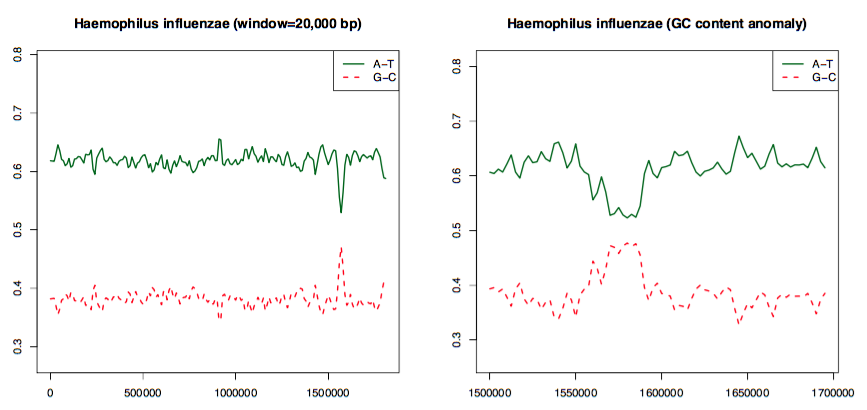
\includegraphics[scale=0.4]{images/01_gc.png}
 	\caption{GC-Content. Anomaly due to an ancient insertion of viral DNA. AT-rich regions denature at lower temperature. The ability to quickly denature DNA facilitates the insertion in the bacterial cell being infected.}
\end{figure}

\subsubsection{Dimer frequencies}

Some dimers are particulary frequent but it is due to have each nitrogenous bases frequent. Need a background model.

\begin{figure}[htp]
	\centering
	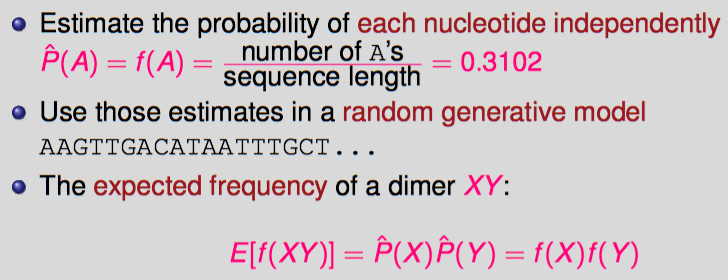
\includegraphics[scale=0.4]{images/02_dimer.png}
 	\caption{Multinomial background model.}
\end{figure}

With the multinomial background model, we can compute the \textbf{odd ratios}: ratio between observed frequency and expected frequency: $\frac{f(XY)}{E[f(XY)]} = \frac{f(XY)}{f(X)f(Y)}$.


The multinomial model is  equivalent to a random permutation of the original sequence: $\frac{f(XY)}{f_{random}(XY)}$.

We can generalize odd ratios to \textbf{k-mers}.

\begin{figure}[htp]
	\centering
	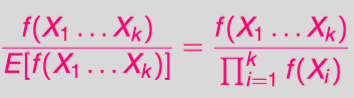
\includegraphics[scale=0.4]{images/03_kmers.png}
 	\caption{k-mers. Useful when looking for frequent patterns of k consecutive characters. But are they informative ? Need a more sophisticated background model, a statistical test to assess signifiance and biological validation.}
\end{figure}

\subsection{Open Reading Frames}

\begin{figure}[htp]
	\centering
	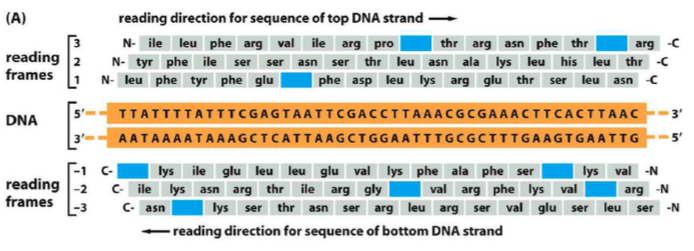
\includegraphics[scale=0.6]{images/04_rf.png}
 	\caption{Reading frames.}
\end{figure}

\subsubsection{Algorithm to find ORF}

\begin{figure}[H]
	\centering
	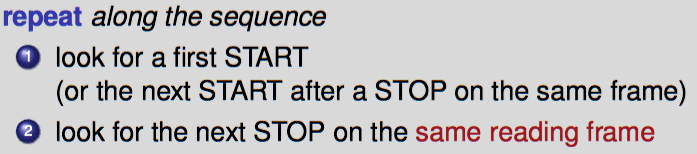
\includegraphics[scale=0.4]{images/05_algo.png}
 	\caption{Need to consider each reading frames (6). After a START, you may find other codons for Met before a STOP: not true START.   An ORF is a longest strech of DNA between a START and a STOP, without being interrupted by another STOP on the same frame.}
\end{figure}

The problem is to have to be sure that the ORF is a coding gene.
\begin{itemize}
	\item The DNA found between STAT and STOP codon might be due to chance: need \textbf{a statistical test procedure};
	\item The ORF might be there but the gene not expressed (trace of past or regulations at transcription/translation levels): need biological validation;
	\item Some gene sequences do not strictly follow the standard ORF structure: need biological validation.
\end{itemize}

\subsubsection{Signifiance assessment}

\begin{figure}[htp]
	\centering
	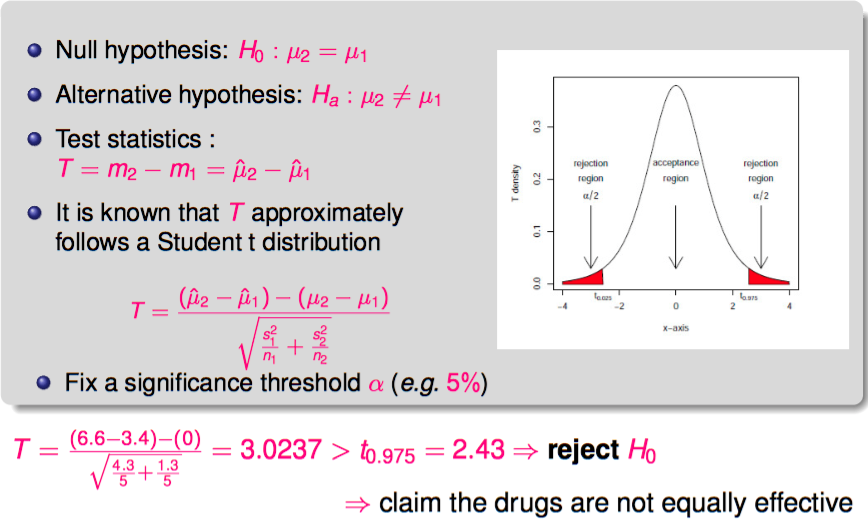
\includegraphics[scale=0.4]{images/06_test.png}
 	\caption{Statistical test. }
\end{figure}

To avoid fixing a signifiance threshold $\alpha$ we can compute the \textbf{p-value} of the test.

\begin{figure}[htp]
	\centering
	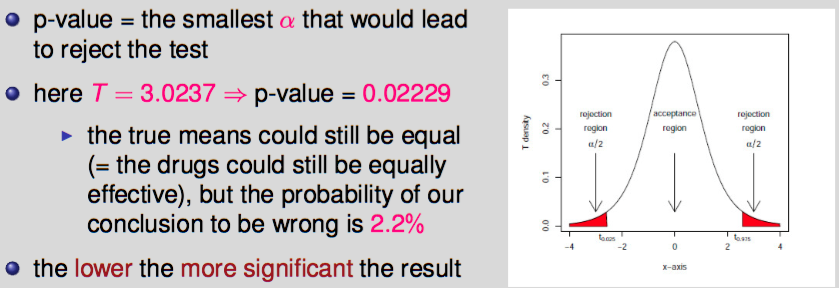
\includegraphics[scale=0.4]{images/07_pval.png}
 	\caption{p-value. }
\end{figure}

We can apply this to ORF.


\begin{figure}[htp]
	\centering
	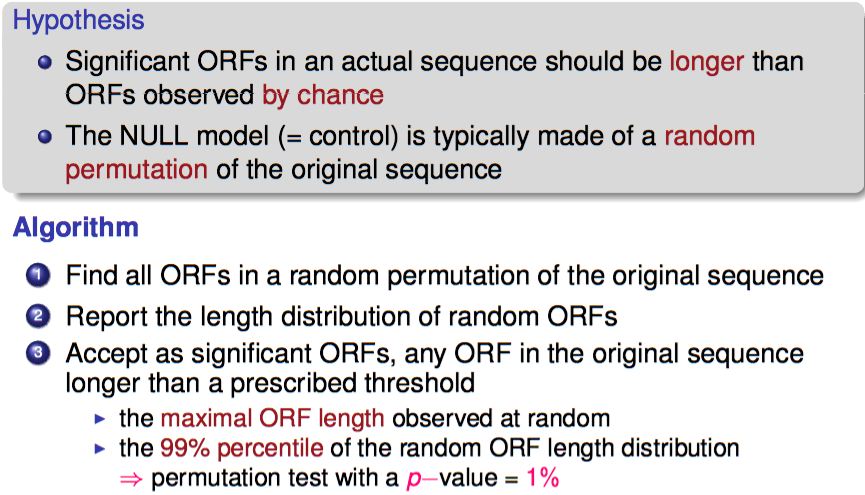
\includegraphics[scale=0.4]{images/08_orf.png}
 	\caption{Algorithm to assess signifiance of ORF.}
\end{figure}

\section{Pairwise Alignments}
%!TEX root = main.tex

\subsection{The problem}

Find a best way to align two sequences including matches, substitutions and possible gaps.

\subsubsection{Gap penalties}

\begin{figure}[H]
	\centering
	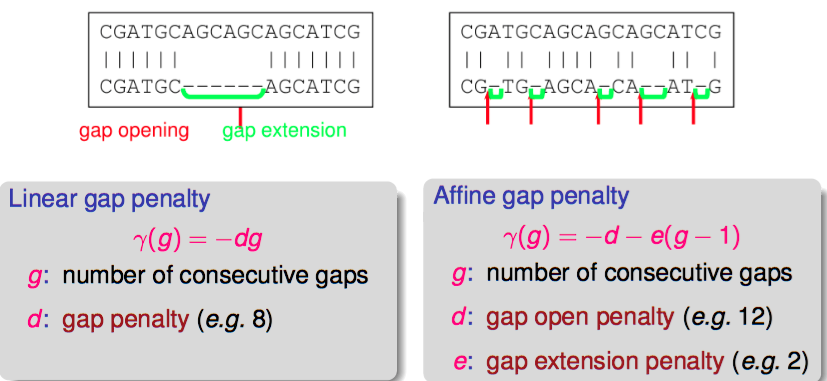
\includegraphics[scale=0.4]{images/09_gap.png}
 	\caption{Gap penalties. Afine is more relevant.}
\end{figure}

\subsubsection{Number of alignements}

The total number alignements is huge ($\frac{4^n}{\sqrt{\pi*n}}$). We need dynamic programming.

\begin{itemize}
	\item We look for maximal cumulative score;
	\item An optimal global alignment is made of optimal alignments between subsequences: decomposition of sub-problems computed only once.
\end{itemize}

\subsection{Global alignment: Needle-Wunsch}


\begin{figure}[htp]
	\centering
	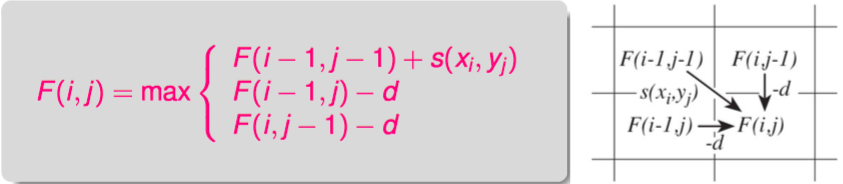
\includegraphics[scale=0.4]{images/10_global.png}
 	\caption{$F(n,m)$ is final alignment score. Need to follow backpointers. $O(n^2)$. }
\end{figure}


\subsection{Local alignment: Smith-Waterman}

\begin{figure}[htp]
	\centering
	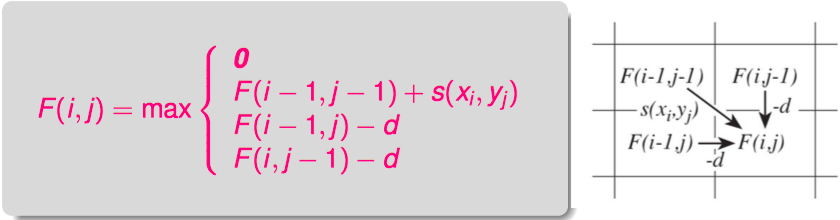
\includegraphics[scale=0.4]{images/11_local.png}
 	\caption{Find maximal $F(i,j)$ and follow backpointers till 0. Need negative scores for strong mismatches. $O(n^2)$.}
\end{figure}

\subsection{Variants}

\subsubsection{Semi-global alignment}
\begin{figure}[H]
	\centering
	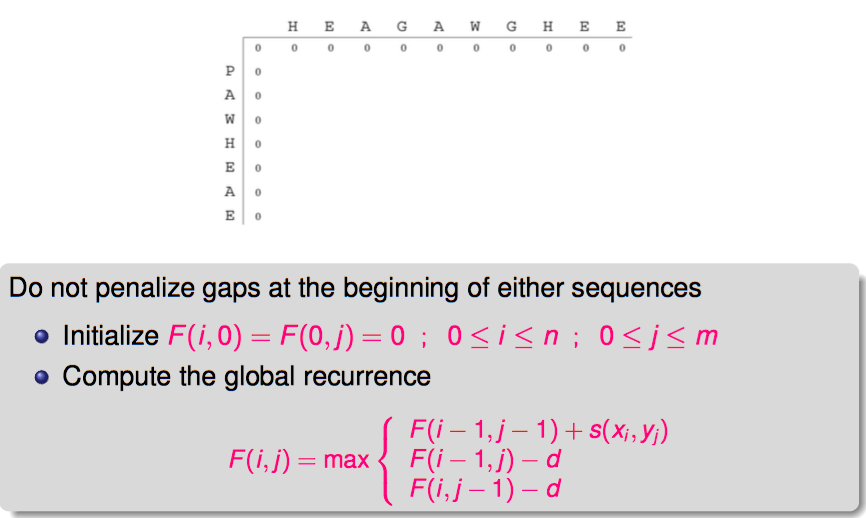
\includegraphics[scale=0.4]{images/12_semi.png}
\end{figure}

\subsubsection{Local alignment with repeats}


\begin{figure}[H]
	\centering
	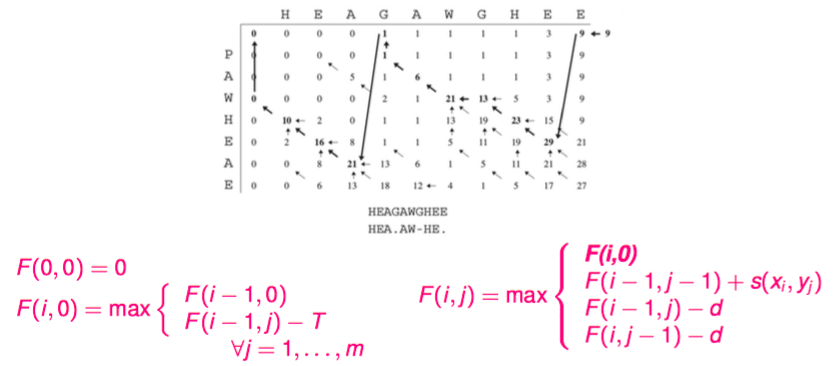
\includegraphics[scale=0.5]{images/13_repeats.png}
	\caption{Look for several matches (subsequences) of y into x. Scoring higher than T.}
\end{figure}

\subsubsection{Affine gap penalty}

\begin{figure}[H]
	\centering
	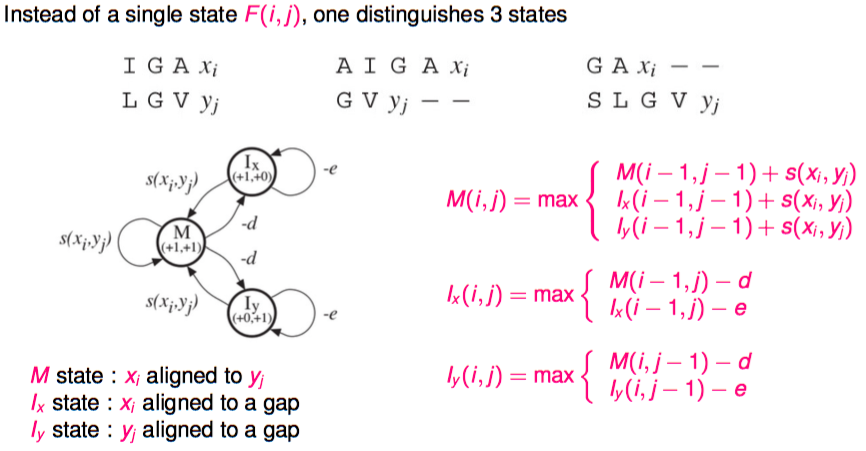
\includegraphics[scale=0.4]{images/14_affine.png}
\end{figure}

\subsection{Signifiance assessment}
\begin{figure}[htp]
	\centering
	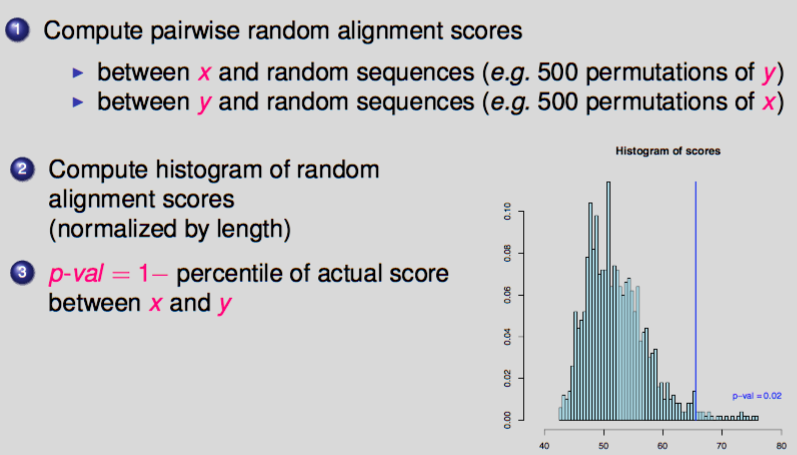
\includegraphics[scale=0.4]{images/15_procedure.png}
	\caption{Procedure.}
\end{figure}

The actual distribution of alginment scores is called \textbf{extreme value distribution}.

\begin{figure}[htp]
	\centering
	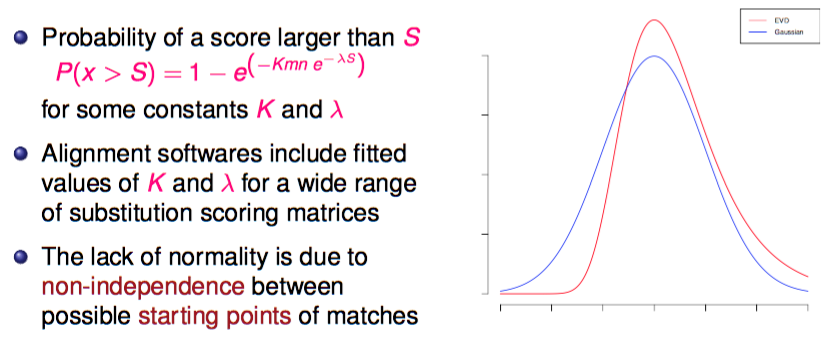
\includegraphics[scale=0.5]{images/16_evd.png}
	\caption{K is a multiplicative factor correcting non independance of possible starting poins for matches. $\lambda$ is a scale parameter.}
\end{figure}

\section{HMMs}
%!TEX root = main.tex

\subsection{An example}

An motivating example is to determine coding or non-coding fragments.

\subsubsection{Baseline approach}


\begin{figure}[htp]
	\centering
	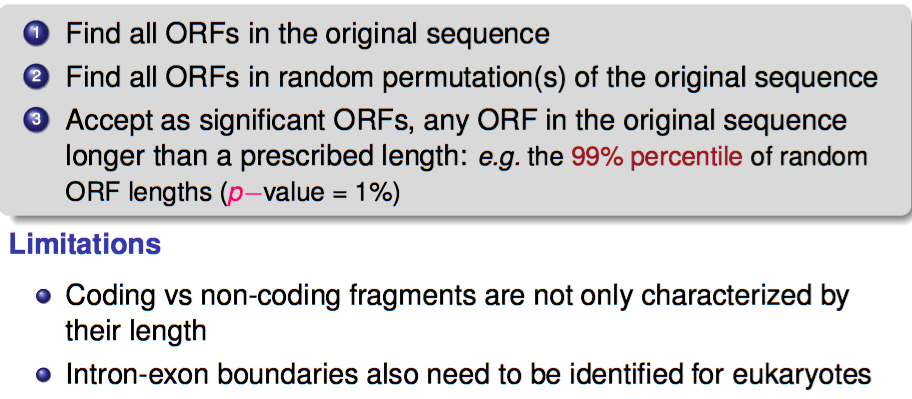
\includegraphics[scale=0.5]{images/17_baseline.png}
\end{figure}

\subsubsection{Alternative approach}

\begin{figure}[htp]
	\centering
	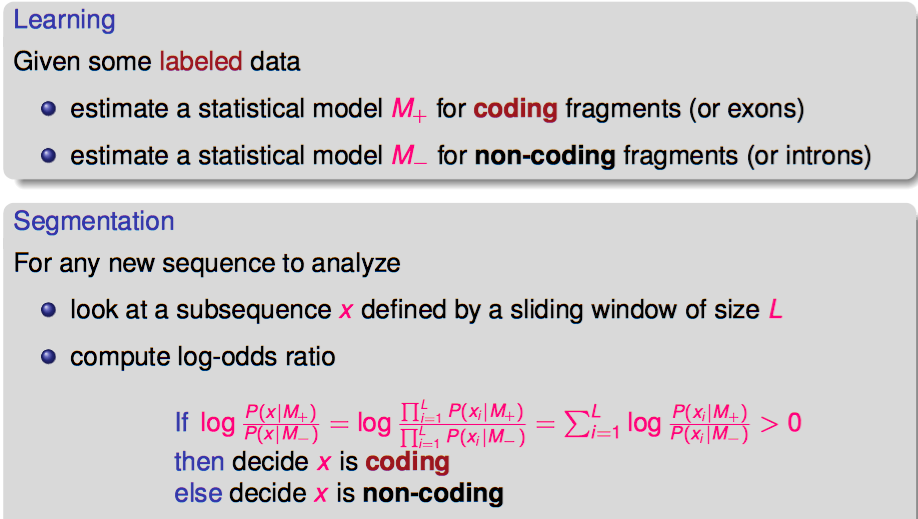
\includegraphics[scale=0.4]{images/18_alt.png}
\end{figure}


\paragraph{Multinomial model}

\begin{center}
  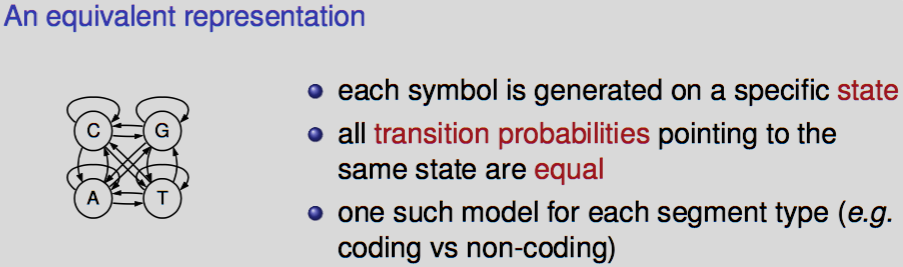
\includegraphics[scale=0.5]{images/19_multi.png}
\captionof{figure}{Two hypothesis: the frequencies are the sames along the different parts of the sequence and each symbol does not depend of surrounding symbols.} 
\end{center}

\newpage
\paragraph{Markov chain}

\begin{center}
	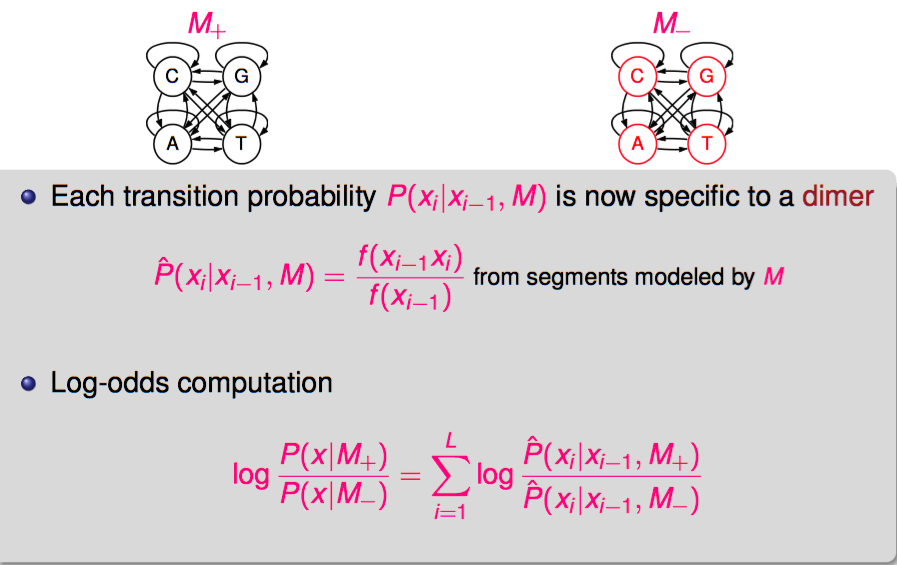
\includegraphics[scale=0.4]{images/20_markov.png}
	\captionof{figure}{First order.}
\end{center}

\begin{center}
	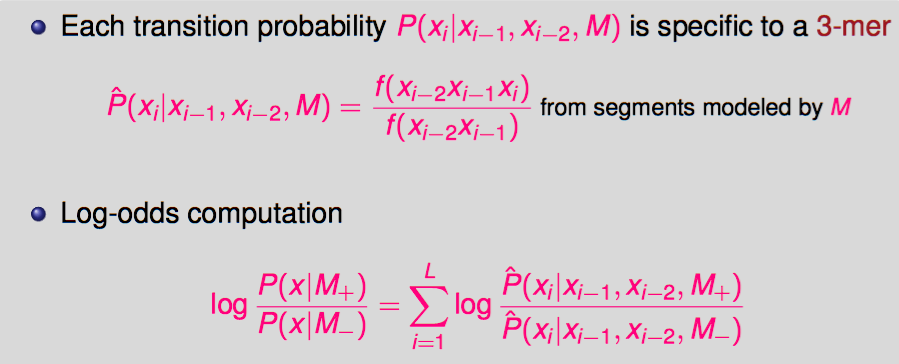
\includegraphics[scale=0.4]{images/21_second.png}
	\captionof{figure}{Second order.}
\end{center}

Limitations of the markov chain approach:
\begin{itemize}
	\item Estimate each MC from well annoted segments;
	\item Gene length variability: sliding window length is arbitrary and we need to find a length that is more relevant: computation expensive;
	\item Eukaryotes: at least three models needed (out of gene, introns, exons).
\end{itemize}
\newpage
\paragraph{Hidden Markov model}

\begin{center}
	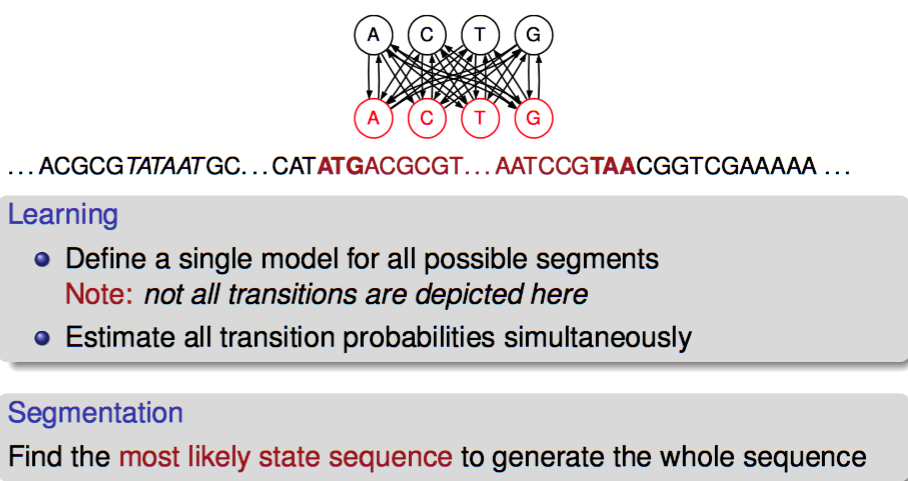
\includegraphics[scale=0.5]{images/22_hmms.png}
	\captionof{figure}{One state for each segment type (coding vs non coding). Transition probabilities, emissions probabilities. States are hidden but their emissions are observed.}
\end{center}

\subsection{Hidden Markov model}

\begin{figure}[htp]
	\centering
	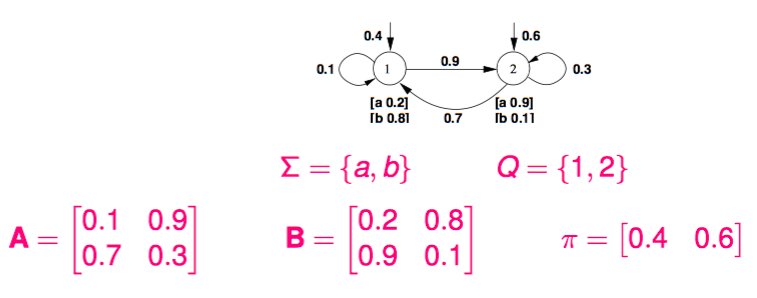
\includegraphics[scale=0.5]{images/24_ex2.png}
\end{figure}

\begin{figure}[htp]
	\centering
	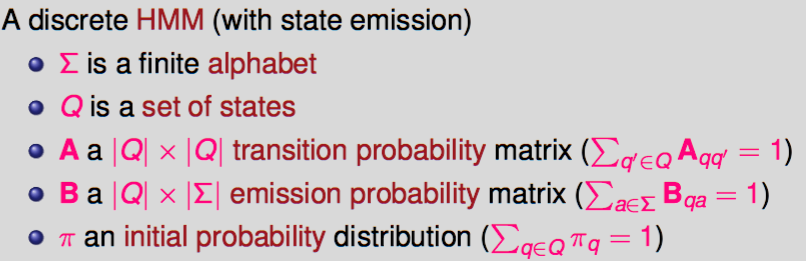
\includegraphics[scale=0.5]{images/23_ex1.png}
	\caption{HMM definition.}
\end{figure}
\newpage
\subsubsection{Path likelihood}

\begin{center}
	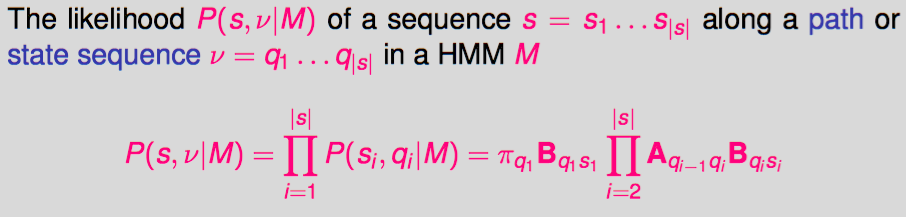
\includegraphics[scale=0.5]{images/25_path.png}
\end{center}

\subsubsection{Probability of generating a sequence}

\begin{figure}[htp]
	\centering
	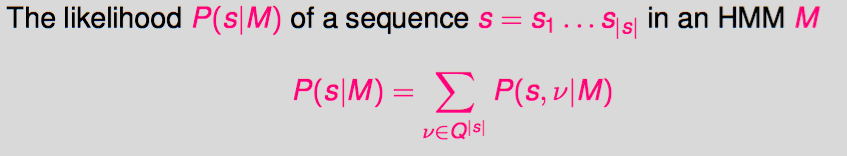
\includegraphics[scale=0.5]{images/26_seq.png}
	\caption{$O(|Q|^{|s|})$ possible state sequences. Q is states and s is sequence.}
\end{figure}

\newpage
\subsubsection{Most likely state sequence}

\begin{figure}[htp]
	\centering
	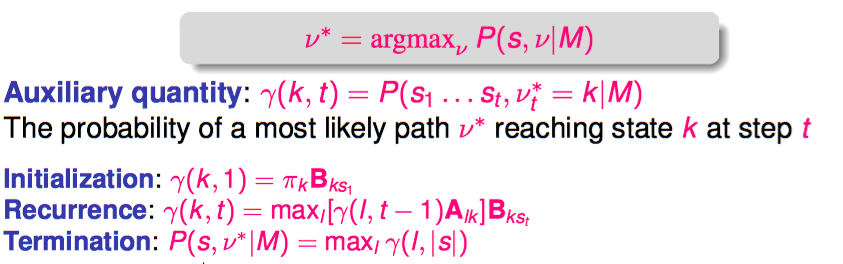
\includegraphics[scale=0.5]{images/27_viterbi.png}
	\caption{Viterbi recurrence.}
\end{figure}

\begin{itemize}
	\item $P(s, v^*)$ gives the probability of the optimal path $v^*$;
	\item Computation are done with log (because too small values);
	\item Complexity: $\Theta(m|s|)$. m is number of HMM transitions;
	\item Path $v^*$ is an alignement between states and words;
	\item $v^*$ can be recovered with the backpointers.
\end{itemize}


\subsubsection{Sequence likelihood}

\begin{figure}[htp]
	\centering
	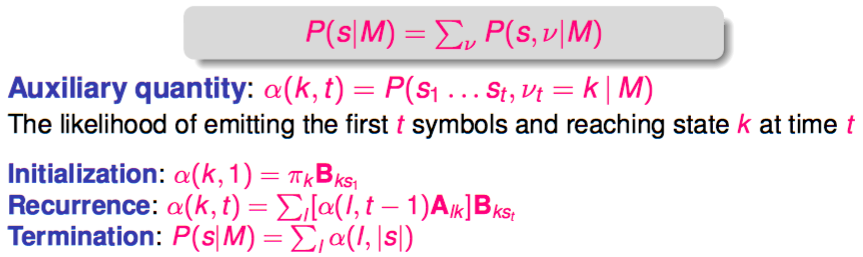
\includegraphics[scale=0.5]{images/28_forward.png}
 	\caption{Forward recurrence, same complexity as viterbi recurrence.}
\end{figure}

\subsection{The learning problem}

Given an HMM structure and several sequences, you must estimate $A$, $B$, $\pi$.


\subsubsection{Supervised learning}

\begin{figure}[H]
	\centering
	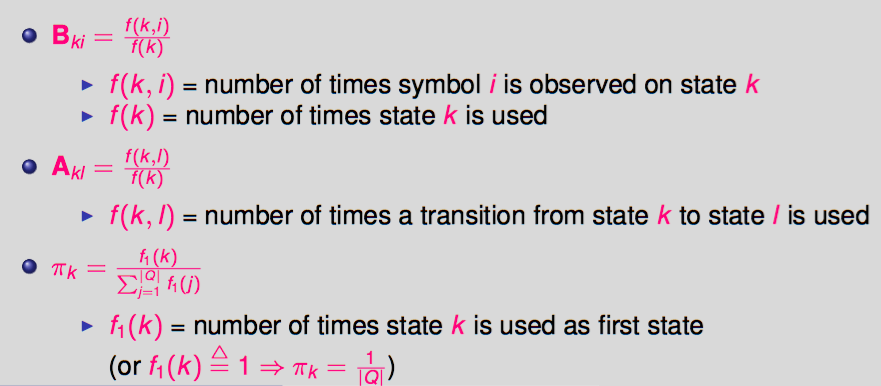
\includegraphics[scale=0.5]{images/29_supervised.png}
 	\caption{Supervised learning.}
\end{figure}

\subsubsection{Unsupervised learning}

The sentences are not annoted. There is two algorithm. The first one is \textbf{Viterbi training}.

\begin{figure}[htp]
	\centering
	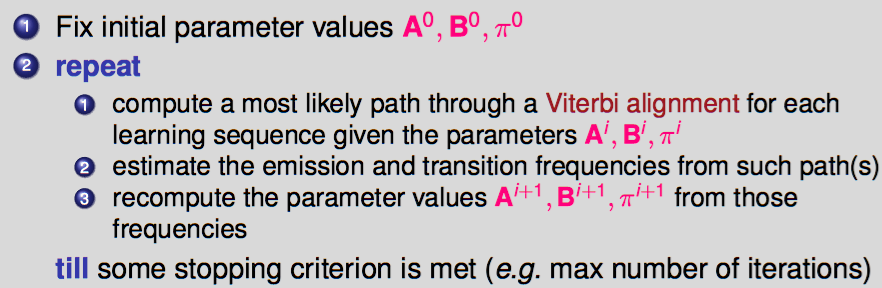
\includegraphics[scale=0.5]{images/30_viterbi.png}
 	\caption{Viterbi learning.}
\end{figure}

The second is \textbf{Forward-Backward} or \textbf{Braaum-Welch} algorithm. Viterbi training is an approximation as it considers that each training sentence is generated along a single path. A more accurate estimation is obtained if one considers all possible paths to generate each sentence.

\begin{itemize}
	\item actual frequencies are replaced by expected frequencies;
	\item   special case of expectation-maximization (EM) procedure
\end{itemize}

Viterbi and Baum-Welch training are both sensitive to parameter initialization.

\subsection{Concrete example}

For CpG islands, we can use a 2-state HMM.

\begin{figure}[htp]
	\centering
	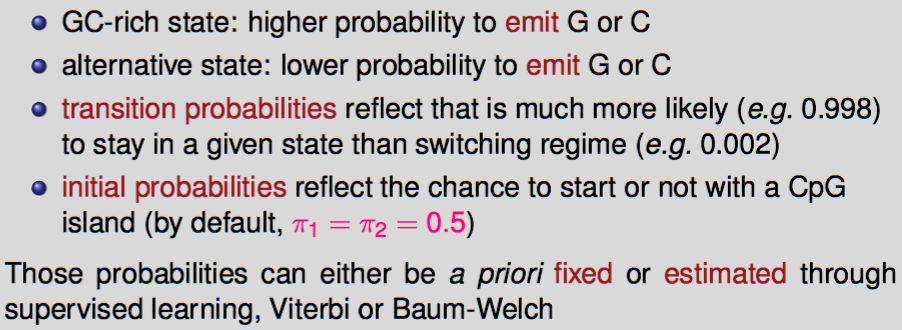
\includegraphics[scale=0.5]{images/31_islands.png}
\end{figure}

\section{Multiple Alignments}
%!TEX root = main.tex

\subsection{The problem}

Align three or more homologuous sequences (globally or localy).

\subsubsection{Scoring}

\begin{figure}[H]
	\centering
	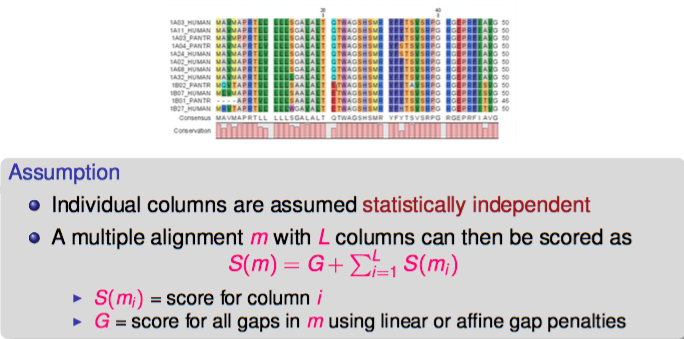
\includegraphics[scale=0.6]{images/32_assumptions.png}
	\caption{Assumptions.}
\end{figure}

\begin{figure}[H]
	\centering
	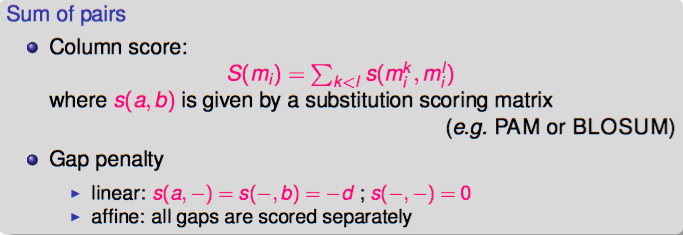
\includegraphics[scale=0.6]{images/33_sums.png}
	\caption{Sum of pairs.}
\end{figure}

\subsection{Dynamic programming}

Optimal alignment between k sequences can be computed with DP. With an average length of $\bar{n}$, the time complexity is $O(2^k \bar{n}^k)$ and the space complexity is $O(\bar{n}^k)$ (hyper cube).

One algorithm which compute optimally the alignement is \textbf{MSA} algorithm ($O(k^2 \bar{n}^2)$: 10 sequences of 200-300 residues in reasonnable time).
\begin{figure}[htp]
	\centering
	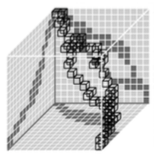
\includegraphics[scale=0.5]{images/34_msa.png}
	\caption{MSA.}
\end{figure}

\begin{itemize}
	\item Compute all pairwise alignments;
	\item Limits the exploration of the hyper cube to regions consitent with those alignments.
\end{itemize}

\textbf{G-MSA} is an optimization: 500 sequences of 236 residues in 10 seconds.

\subsubsection{Progressive alignment methods (greedy heuritic)}

\begin{figure}[htp]
	\centering
	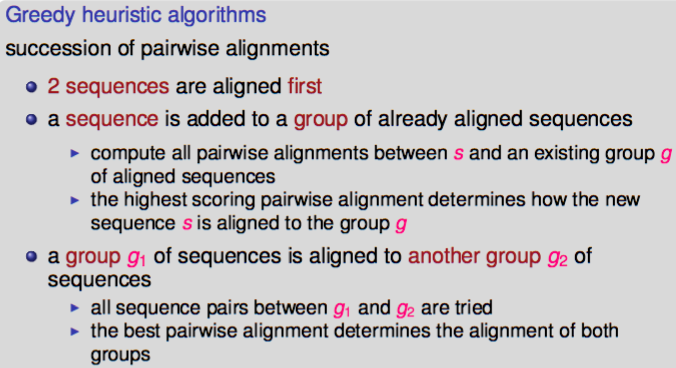
\includegraphics[scale=0.5]{images/35_greedy.png}
	\caption{Greedy heuritic.}
\end{figure}

There are some limitations:
\begin{itemize}
	\item the degree of sequence conservation at each position should be taken into account;
	\item mismatches at highly conserved positions should be more penalized;
	\item the order in which sequences are incorporated in the multiple alignment matters.
\end{itemize}
\newpage
\paragraph{ClustalW}

\begin{center}
	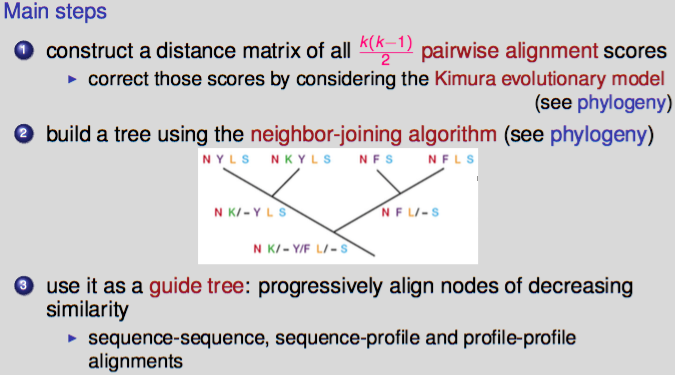
\includegraphics[scale=0.5]{images/36_clustalW.png}
\end{center}

There can be further heuristics:
\begin{itemize}
	\item \textbf{position specific gap open penalties with decreased penalties} wherever other gaps have been found amoung already aligned sequences;
	\item gap penalties are also decreased or increased based on a large collection of \textbf{structural alignments};
	\item the guide tree may be ajusted \textbf{on the fly} to defer a low scoring alignment until more profile information has been accumulated.
\end{itemize}



\section{Profile HMMs}
%!TEX root = main.tex

\subsection{Motivations}

\begin{itemize}
	\item multiple alignments are most often based on pairwise alignments;
	\item a new sequence x may be only distantly and locally related to each sequence in a known family (biological question): all pairwise alignments between x and each family members will look poor. We need to model \textbf{statistical features} shared by the family members;
	\item computing the alignment between x and a probabilistic model of the family may be much \textbf{more efficient computationally}.
\end{itemize}

\subsection{Position specific scoring matrices}

\begin{figure}[H]
	\centering
	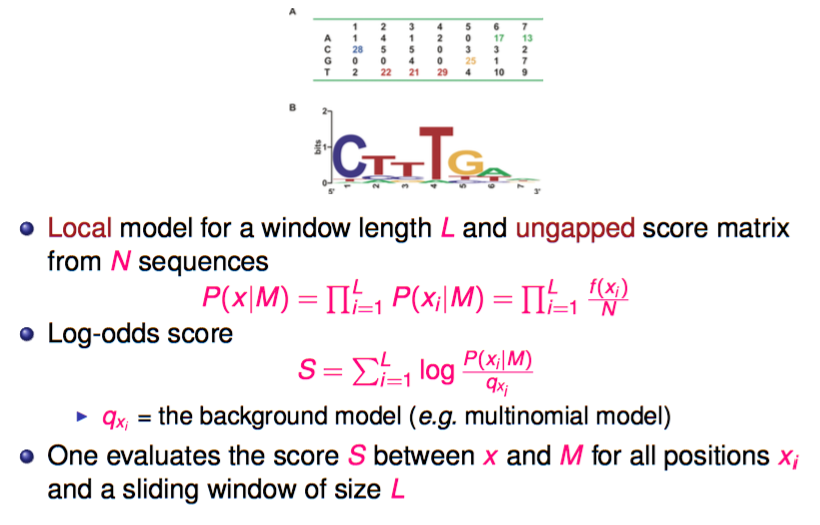
\includegraphics[scale=0.5]{images/37_pssm.png}
	\caption{PSSMs are very simple HMMs. $P(x_i|M)$ are emission probabilities on match state. Transition probabilities are equal to 1. But we need to account for possible gap and avoid a prescribed window length.}
\end{figure}

\begin{figure}[H]
	\centering
	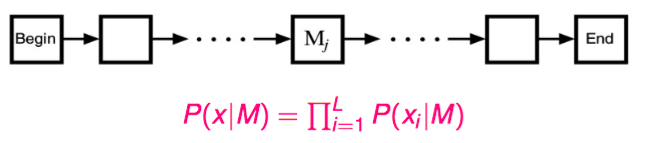
\includegraphics[scale=0.6]{images/40_pssm.png}
\end{figure}

\subsection{Full profile HMMs}

\subsubsection{Adding insert states}

\begin{figure}[H]
	\centering
	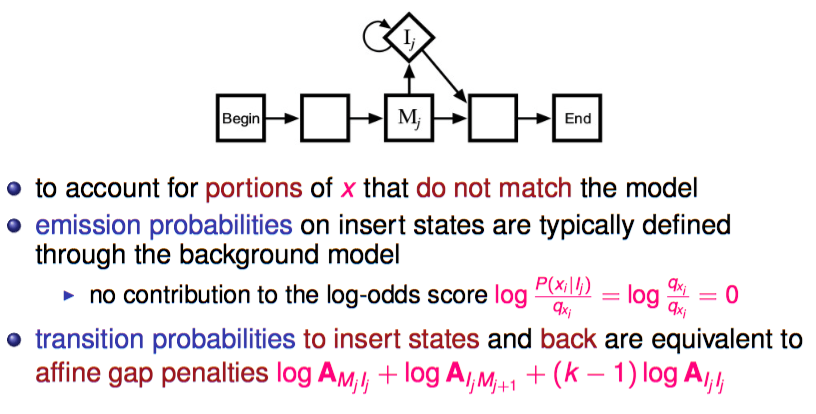
\includegraphics[scale=0.5]{images/38_insert.png}
\end{figure}

\subsubsection{Adding delete states}

\begin{figure}[H]
	\centering
	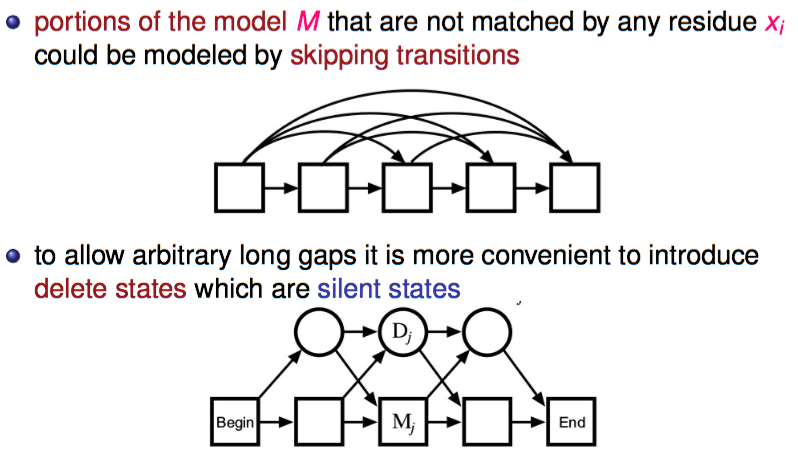
\includegraphics[scale=0.5]{images/39_delete.png}
	\caption{More convenient because less transitions.}
\end{figure}

\subsubsection{A full profile HMM}

\begin{figure}[H]
	\centering
	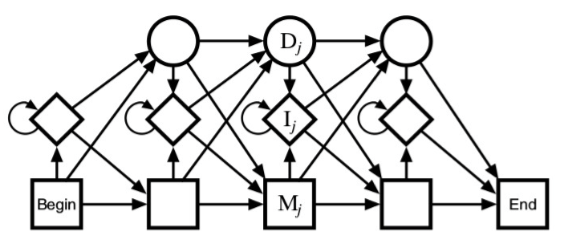
\includegraphics[scale=0.6]{images/41_phmm.png}
	\caption{Parameters are: value of the probabilities and length. Begin, End and D states are silent.}
\end{figure}

\subsubsection{Deriving a pHMM from a multiple alignement (Supervised)}


\begin{figure}[H]
	\centering
	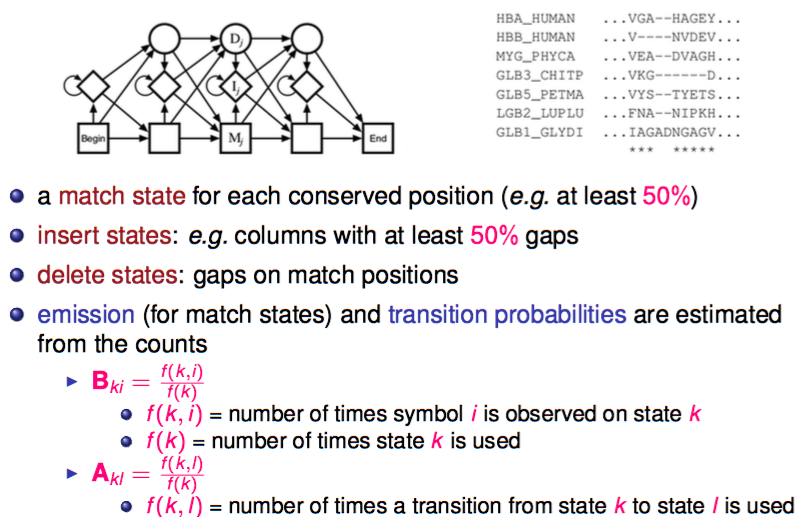
\includegraphics[scale=0.5]{images/42_deriving.png}
\end{figure}

But the initial multiple alignement could have some probabilities equal to zero: we need \textbf{smoothing}.

\begin{figure}[htp]
	\centering
	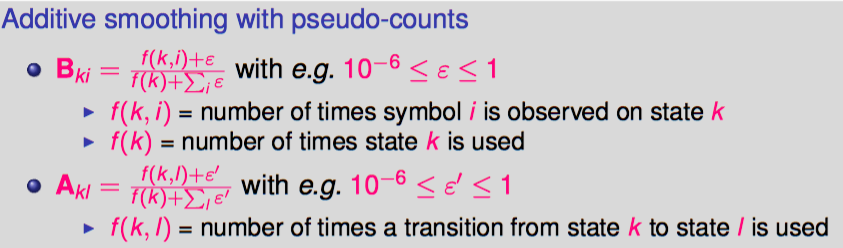
\includegraphics[scale=0.5]{images/43_smoothing.png}
\end{figure}

\subsubsection{Unsupervised learning}

No need for an initial multiple alignment (only unaligned sequences).

\begin{figure}[htp]
	\centering
	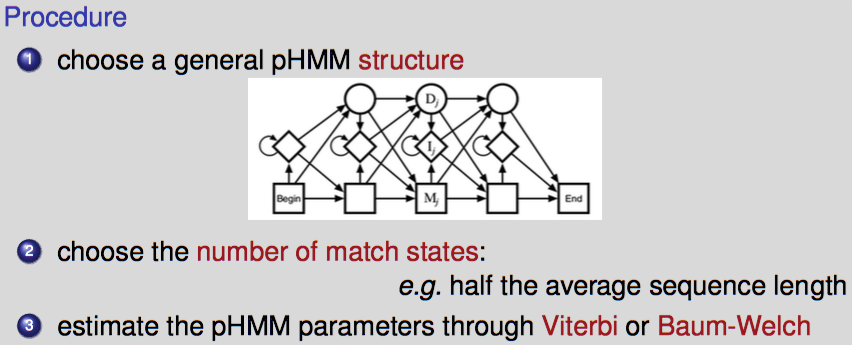
\includegraphics[scale=0.5]{images/44_unsupervised.png}
\end{figure}

\subsubsection{Matching a sequence to a pHMM a.k.a. viterbi recurrence}


\begin{figure}[H]
	\centering
	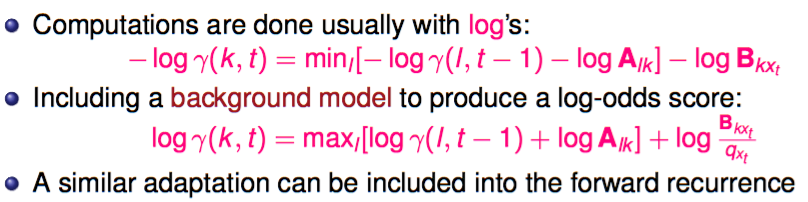
\includegraphics[scale=0.5]{images/45_viterbi.png}
\end{figure}

\newpage

\subsubsection{For non-global alignments}


\begin{figure}[H]
\begin{adjustwidth}{-2cm}{}
\centering
\begin{minipage}{.47\linewidth}
  \centering
  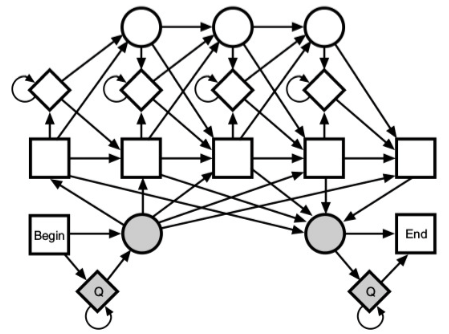
\includegraphics[scale=0.5]{images/46_nglobal.png}
  \caption{Local alignment (S-W style). Non-conserved fragments are modeled through flanking insert states using the backgroud emission probabilities $q_a$. Their loop have high probabilities. Flanking delete states allow for starting or ending the profile at any point and reduce number of transitions.}
\end{minipage}%
\hspace{0.5cm}
\begin{minipage}{.47\linewidth}
  \centering
  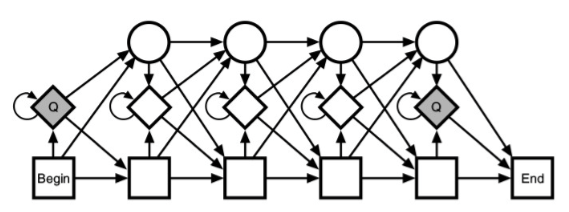
\includegraphics[scale=0.5]{images/47_nglobal.png}
  \caption{Set all the transition probabilities from the left flanking state to different start points. Force the match on the compelte profile.}
\end{minipage}
\end{adjustwidth}
\end{figure}

\begin{figure}[htp]
	\centering
	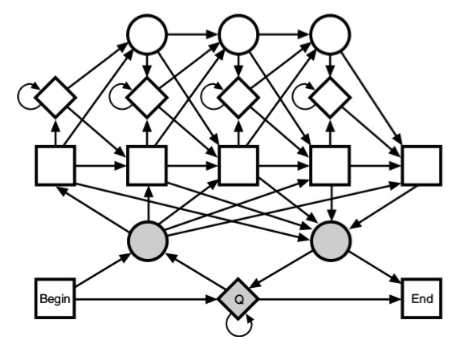
\includegraphics[scale=0.5]{images/48_nglobal.png}
	\caption{Allow repeated matches to subsections of the profile.}
\end{figure}




\section{Large Scale Gene Expression Analysis}
%!TEX root = main.tex

\subsection{Introduction}

DNA Microarrays measure the level of expression of all genes in a signle experiment. Data measurements $\rightarrow$ Preprocess and sample normalization $\rightarrow$ Gene selection and sample classification $\rightarrow$ Diagnosis, prognosis or prediction of the reponse to a treatment.

The \textbf{gene selection} (supervised learning) to find a subset of genes to predict the response of new samples. There are some \textbf{objectives}:
\begin{itemize}
	\item Insight into the data and the predictive model;
	\item Link between data analysis and medical expert;
	\item Biological validation;
	\item Reduce financial cost.
\end{itemize}

There are some \textbf{difficulties}:
\begin{itemize}
	\item Measurements are noisy;
	\item Gene expression varies due to many factors;
	\item Financial cost;
	\item Small n large p problem.
\end{itemize}

\subsection{Preprocessing}

\subsubsection{Summarization}

Define a single probeset expression level from the various probe intensities. There are popular techniques: MAS 5.0, RMA, GC-RMA. 
\begin{itemize}
	\item background adjustment: optical noise correction, probe affinity adjustment (influenced by the GC content), RMA ignores the MM probes;
	\item sample normalization: quantiles should be stable across samples, after conversion to log intensities for (GC-)RMA;
	\item summarization: median polish.
\end{itemize}

\subsubsection{Feature normalization}

Make sure that each gene (probeset) has roughly the same expression range across all samples and then do a \textbf{Z-score normalization}: Replace $x_{i,j}$ by $\frac{x_{i,j} - \mu_j}{s_j}$. $\mu_j$ is the mean level of expression of probeset j over the training samples and $s_j$ is the tandard deviation.

\subsubsection{Distance between expression values}

\begin{figure}[H]
	\centering
	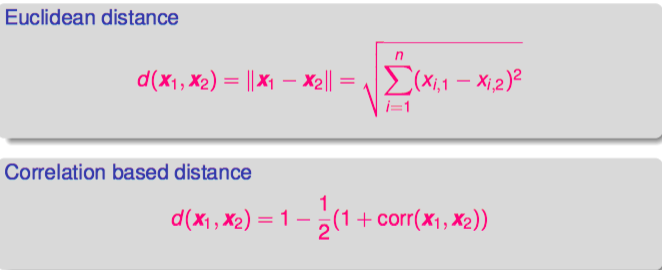
\includegraphics[scale=0.5]{images/51_distance.png}
\end{figure}

\paragraph{Pearson correlation}

\begin{center}
	\includegraphics[scale=0.6]{images/52_pearson.png}
\end{center}

\paragraph{Pitfalls with correlation measure}

\begin{center}
	\includegraphics[scale=0.6]{images/53_outliers.png}
	\captionof{figure}{Correlation is sensitive to outliers.}
\end{center}

\begin{center}
	\includegraphics[scale=0.4]{images/54_linear.png}
	\captionof{figure}{Correlation measures \textbf{linear} dependence.}
\end{center}


\paragraph{Spearman's rank correlation}

This correlation is less sensitive to outliers (but still measure linear dependence).
\begin{itemize}
	\item Replace feature value by feature value rank across observations;
	\item Compute pearson correlation between rank vectors.
\end{itemize}

\subsection{Unsupervised learning}

\begin{figure}[H]
	\centering
	\includegraphics[scale=0.4]{images/50_unsupervised.png}
	\caption{Objective is to find cluster of genes that share similar profile.}
\end{figure}


\begin{figure}[H]
	\centering
	\includegraphics[scale=0.55]{images/55_agglo.png}
	\caption{Agglomerative hierarchical clustering.}
\end{figure}
There are different distance measure between the clusters.

\begin{figure}[htp]
	\centering
	\includegraphics[scale=0.6]{images/56_measure.png}
\end{figure}

\textbf{UPGMA} algorithm is with average-link measure. Used in phylogeny.


\subsection{Supervised learning}

\begin{figure}[htp]
	\centering
	\includegraphics[scale=0.6]{images/49_supervised.png}
	\caption{p input dimensions, n samples, y is binary, natural or real. THe goal is to find the most discriminating genes for the prediction of the class of any new sample.}
\end{figure}

\subsubsection{Filters}

\begin{figure}[H]
	\centering
	\includegraphics[scale=0.6]{images/57_filters.png}
	\caption{Use only training data and class labels during the features selection step and then train a single classifier taking the selected features as inputs. It is the less computive approach.}
\end{figure}

\paragraph{Non-specific filtering}

Keep only genes with the larger variances (top 25\%) because they are discriminating (do it before normalization to unit variance).


\paragraph{Fold changes}

\begin{center}
	\includegraphics[scale=0.6]{images/60_fold.png}
	\captionof{figure}{Keep genes with larger fold changes between both conditions. Not a good filters because discriminating genes with large difference but small ratio are missed.}
\end{center}

\paragraph{t-Test relevance index}

\begin{center}
	\includegraphics[scale=0.6]{images/61_test.png}
	\captionof{figure}{$J(x)$ is the distance between feature and average feature value in \textbf{each class}. p-values assess the signifiance of the difference between the two class means. A feature is selected if its associated p-value is below a prescribed theshold.}
\end{center}

\subparagraph{Alternatives of the simple t-Test}
\begin{itemize}
	\item Mann-Whitney rank test is an alternative \textbf{non-parametric} test;
	\item ANOVA is a generalization of the t-Test with \textbf{multi-class} (bigger than 2);
	\item Pairwise t-Tests \textbf{between one class and the others};
	\item Kruskal-Wallis is a generalization of M-W (\textbf{non parametric multi class}).
\end{itemize}

\paragraph{Multiple test correction}

It is possible to conclude that the mean expression values among the 2 classes are significantly different for a given gene while they are not. If the test is performed 50000 times and $\alpha = 0,05$, we are expected to wrongly select $50000*0,05=2500$ genes. We need correction.

\subparagraph{Bonferoni correction}

Divide the critical value by the number of tests $n_t$ performed ($\frac{0,05}{50000}$). Tends to select no features.

\subparagraph{False Discovery Rate correction}

\begin{center}
	\includegraphics[scale=0.6]{images/62_fdr.png}
	\captionof{figure}{If $p_{n_t} < 0,05$ FDR select all the features. Only the selection threshold is changed.}
\end{center}


\newpage
\paragraph{Feature ranking with mutual information}

\begin{center}
	\includegraphics[scale=0.6]{images/63_mutual.png}
	\captionof{figure}{A feature X is more relevant if its mutual information with the class value is higher. If X tend to bring no info to predict Y: $I(X;Y) \rightarrow 0$. $I(X;Y) = 0$ if X and Y independent.}
\end{center}


Those are univariate filters. We can use mutual information to select several variables at a time. 

\paragraph{Maximum relevance minimum redondancy}
\begin{center}
	\includegraphics[scale=0.6]{images/64_maxmin.png}
\end{center}

\paragraph{Conclusion}

Filters is the cheapest approach and is useful when we have large number of features. Univariate filters ignore interactions between genes. 

\subsubsection{Wrappers}

\begin{figure}[H]
	\centering
	\includegraphics[scale=0.6]{images/58_wrappers.png}
	\caption{Train a classifier on several subsets of all possible features ($O(2^p)$ different subsets). Exhaustive search is impossible, use feature rankin or f/b selection. Select the feature set that optimize the performance of the trained classifier.}
\end{figure}

\begin{figure}[H]
\centering
\begin{minipage}{.5\textwidth}
  \centering
  \includegraphics[scale=0.5]{images/65_uni.png}
  \caption{Univariate feature ranking.}
\end{minipage}%
\begin{minipage}{.5\textwidth}
  \centering
  \includegraphics[scale=0.5]{images/66_multi.png}
  \caption{Multivariate Forward (bottum-up, nothing to all) or Backward (top-down, all to nothing) selection.}
\end{minipage}
\end{figure}

The search order matters. If you can afford the computational cost of multivariate selection, you can do an embedded approach.


\subsubsection{Embedded approaches}

\begin{figure}[H]
	\centering
	\includegraphics[scale=0.6]{images/59_embedded.png}
	\caption{Feature selection and classifier estimation is the same \textbf{combined optimization process}. We include the classifier optimization in the feature selection process. The most computing expensive.}
\end{figure}

\paragraph{Linear discriminats}

\begin{center}
	\includegraphics[scale=0.5]{images/67_linear.png}
	\captionof{figure}{The problem is there can be several hyperplane.}
\end{center}
\newpage
\paragraph{Linear Support Vector Machines}

\begin{center}
	\includegraphics[scale=0.6]{images/68_svm.png}
	\captionof{figure}{SVM. Need to find the maximal margin.}
\end{center}

\paragraph{Recursive feature Elimination}

\begin{center}
	\includegraphics[scale=0.5]{images/69_rec.png}
\end{center}



\section{Inference of Gene Regulatory Network}
%!TEX root = main.tex
It's the set of all transcription interactions in a cell. There is some regulator (transcription factor) and regulated gene (target). 

\begin{landscape}

\begin{figure}
\begin{tabular}{|c|c|}
  \hline
	\includegraphics[scale=0.5]{images/70.png}
  & 
	\includegraphics[scale=0.5]{images/71.png}
 \\ \hline
	\includegraphics[scale=0.5]{images/72.png}
  & 
	\includegraphics[scale=0.5]{images/73.png}
  \\
  \hline
\end{tabular}

\end{figure}

\end{landscape}

%----------------------------------------------------------------------------------------
%	BIBLIOGRAPHY
%----------------------------------------------------------------------------------------

%----------------------------------------------------------------------------------------

\end{document}